% ---------
%  Compile with "pdflatex hw0".  
% --------
%!TEX TS-program = pdflatex

\documentclass[letterpaper,11pt]{article}
\usepackage{jeffe,handout,graphicx}
\usepackage{fancyhdr}
\usepackage{comment}

% ---------
% Input file uses Unicode's UTF-8 encoding
% ---------
%!TEX encoding = UTF-8 Unicode
\usepackage[T1]{fontenc}
\usepackage[utf8]{inputenc}

% ---------
%  The next several lines (up to the line of =='s) change the default text
%  and math fonts and make a few other minor cosmetic changes.  If you get
%  any error messages related to these packages, just comment them out.
%         -- Jeff
% --------
%\usepackage[charter]{mathdesign}
% \def\sfdefault{fvs}
% \def\ttdefault{fvm}
% \SetMathAlphabet{\mathsf}{bold}{\encodingdefault}{\sfdefault}{b}{\updefault}
% \SetMathAlphabet{\mathtt}{bold}{\encodingdefault}{\ttdefault}{b}{\updefault}
% \SetMathAlphabet{\mathsf}{normal}{\encodingdefault}{\sfdefault}{\mddefault}{\updefault}
% \SetMathAlphabet{\mathtt}{normal}{\encodingdefault}{\ttdefault}{\mddefault}{\updefault}
% \usepackage{microtype}
% ---------
%  End of cosmetics.
% --------

% ---------
%  Redefine suits
% --------
\usepackage{pifont}
\def\Spade{\ding{171}}
\def\Heart{\textcolor{Red}{\ding{170}}}
\def\Diamond{\textcolor{Red}{\ding{169}}}
\def\Club{\ding{168}}


\newtheorem{lemma}{Lemma}
\newtheorem{definition}{Definition}

\newcommand{\hdr}[2]{
   \newpage\setcounter{page}{1}
   \lhead{\fancyplain{}{\textbf{#1}}}
   \rhead{\fancyplain{}{\textbf{#2}}}
   \cfoot{\fancyplain{}{\thepage}}
}

% =========================================================
\begin{document}
\pagestyle{fancy}
\fancyhf{}
\hdr{CS 573 HW0}{Zigang Xiao (zxiao2) HW0 \#1}
 
\small\sf	% typeset excetps from problems in a different, smaller font

\begin{center}
\EMPH{I understand the course policies.}
\end{center}

\begin{enumerate}
\item
\begin{enumerate}\itemsep 2ex plus 0.1fil

\item
Solve the recurrences.

\begin{solution}
\begin{align*}
	A(n) &= \Theta(4^n) \\
	B(n) &= \Theta(n^3) \\
	C(n) &= \Theta(n^2) \\
	D(n) &= \Theta(n^{\log_3 2}) \\
	E(n) &= \Theta(3^{n/2}) \\
\end{align*}
\end{solution}

\item
Sort the functions from asymptotically smallest to asymptotically largest, indicating ties if any.

\begin{solution}
\begin{align*}
		\sqrt{\lg n}
	& \ll
		\lg{n} \\
	& \equiv
		\lg{\sqrt{n}} \\
	& \ll
		7^{\sqrt{\lg n}} \\
	& \ll
		\sqrt{n} \\             % how to compare this and above one?
	& \equiv
		\sqrt{\lg(7^n)} \\
	& \equiv
		\lg(7^{\sqrt{n}}) \\
	& \ll
		7^{\lg \sqrt{n}} \\
	& \equiv
		\sqrt{7^{\lg{n}}} \\
	& \ll
		\lg \sqrt{7^n} \\
	& \equiv
		\lg (7^n) \\
	& \equiv
		n \\
	& \ll
		7^{\lg{n}} \\
	& \ll
		7^{\sqrt{n}} \\
	& \ll
		\sqrt{7^{n}} \\
	& \ll
		7^{n}
	\end{align*}
\end{solution}

\end{enumerate}

%----------------------------------------------------------------------
\def\symbol#1{\textbf{\texttt{#1}}}
\newpage
\hdr{CS 573 HW0}{Zigang Xiao (zxiao2) HW0 \#2}
\item
\begin{enumerate}
\item
List the nodes in Prof. della Giungla's tree in the order visited by a \emph{preorder} traversal. 

\begin{solution}
  \symbol{S Q V I R T Z A P H O D B X F L E G M N Y C K}
\end{solution}

\item
Draw Prof. della Giungla's tree.

\begin{solution}~

\begin{center}
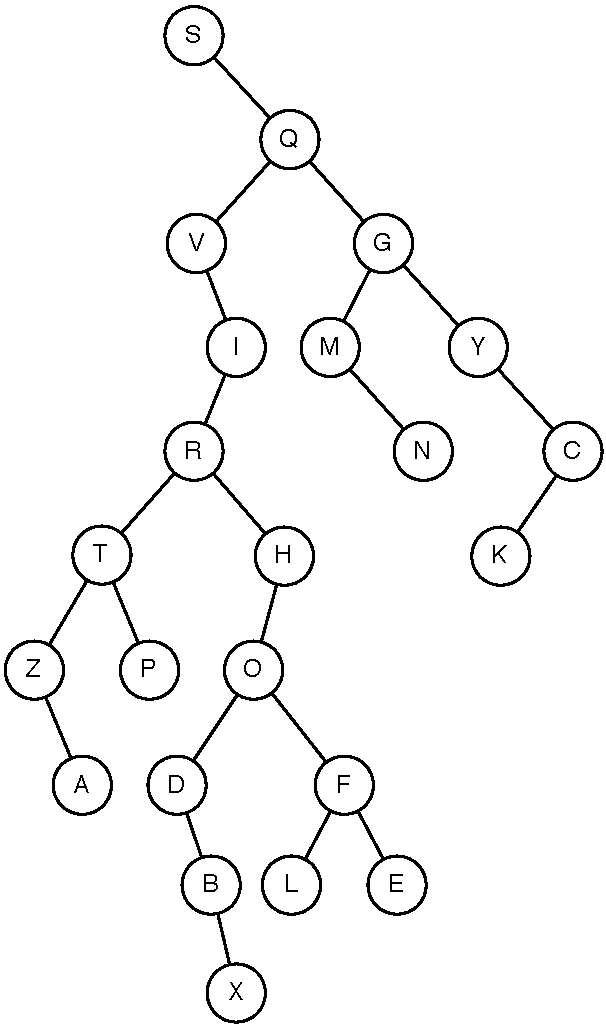
\includegraphics[width=0.6\textwidth]{Fig/tree.pdf}
\end{center}
\end{solution}

\end{enumerate}

%----------------------------------------------------------------------
\newcommand{\HtR}{\textsc{\textrm{HighestToRight}}}
\newcommand{\RmA}{\textsc{\textrm{RightmostAbove}}}
\hdr{CS 573 HW0}{Zigang Xiao (zxiao2) HW0 \#3}
\item
Describe a data structure that stores a set of $n$ points in the plane and
supports the queries \HtR{} and \RmA.

\begin{solution} 
We will first give a definition as follows:
  \begin{definition}
    A point $p=(p_x,p_y)$ is dominated by a point $q=(q_x,q_y)$ if and only if 
    $p_x<q_x$ and $p_y<q_y$.
  \end{definition}

For each point $p$ in $S$, we remove it from $S$ if it is dominated by some
point $q$.  After we remove all such points, we get a set $S'$ of these
remaining points.  Any two points in $S'$ will not dominate each other. Then,
we sort these points according to their $x$-coordinates and store them in an
array.

To make a query \HtR$(\ell)$, we use a binary
search to find an element $p=(i,j)$ in the array such that $l\leqslant i$ and
$p$ is closest to $l$ in $x$-direction. Return this point for the query. If no
such point can be found, i.e., $l$ is greater than the $x$-coordinate of the
last point in the array, return $\textsc{None}$.

Similary, to make a query \RmA$(\ell)$, use
binary search to find an element $p=(i,j)$ such that $l\leqslant j$ and $p$ is
closest to $l$ in $y$-direciton.\\

\noindent \textbf{Correctness:}
We first prove that a point $p$ that is dominated by some other point $q$
cannot be the output of \HtR.  Otherwise, $q$ will be a better point 
than $p$ since $q$ is higher than $p$ and has a greater $x$-coordinate.
Similarly this is true for \RmA. In other words, all of the possible return 
values of the algorithm will be in $S'$.

Next, we prove the correctness of the algorithm. For \HtR, the point $p$ we find
that is closest to $l$ in $x$-coordinate must have the highest $y$-coordinate.
Assume that it is not true and there is a point $q$ that has the highest
$y$-coordinate and whose $x$-coordinate is greater than or equal to $l$, but it
is not closest to $l$ in $x$-coordinate. Then, $q$ will then dominate any point
$p$ that has smaller $x$-coordinate than $q$.  Hence, $q$ will be the point 
that is closest to $l$ in $x$-coordinate. This causes contradiction.
Similarly, we can prove the correctness of our algorithm for \RmA. \markatright{\QED}\\

\noindent \textbf{Analysis:}
The data structure used here is an array that has at most $n$ elements in the 
worst case that no point dominates others, and thus use $O(n)$ space.  
The query uses only a binary search and thus runs in $O(\log{n})$ time.  
\end{solution}

%----------------------------------------------------------------------
\hdr{CS 573 HW0}{Zigang Xiao (zxiao2) HW0 \#4}
\item
Prove that for any arithmetic expression tree, there is an equivalent arithmetic expression tree in normal form.

\begin{solution}
We prove the statement by induction. 
\begin{proof}
Let $n$ be an arbitrary non-negative integer.
Assume that for all arithmetic expression trees with depth $l<n$, 
there is an equivalent arithmetic expression tree in normal form. 
\begin{itemize}
  \item If $n=0$, it is trivially true.
  \item If $n \geqslant 1$, for any arithmetic expression tree with depth $n$, 
    there are two subcases to consider:
    \begin{itemize}
      \item If the root node is a $+$-node, the inductive hypothesis shows that
	both subtrees of this node has a arithmetic expression tree in normal
	form.  So this tree has an equivalent arithmetic expression tree in
	normal form because the root node is a $+$-node and will not introduce
	a $\times$-node parent.
      \item If the root node is a $\times$-node, we first observe that we can
	distribute the $\times$-node as shown in Figure~\ref{fig:expr}.  The
	heights of the subtrees $A$, $B$, $C$ and $D$ are at most $n-2$.  After
	distribution, the heights of the subtrees $A-\times-C$, $A-\times-D$,
	$B-\times-C$ and $B-\times-D$ are $n-1$.  By inductive hypothesis they
	have equivalent arithmetic expression trees in their normal forms.
	Furthermore, according to the definition of normal form, all $+$-nodes
	in the normal form of an arithmetic expression tree will be in the
	higher level of the tree than the $\times$-nodes.  Hence, we can
	transform these four subtrees to their normal form such that all the
	$+$-nodes are moved above the $\times$-nodes.  Then, the resulting tree
	is also in normal form since all the $+$-nodes are still above the
	$\times$-nodes.
    \end{itemize}
\end{itemize} 
In conclusion, the statement holds for all cases.
\end{proof}

\begin{figure}[hb]
  \centering
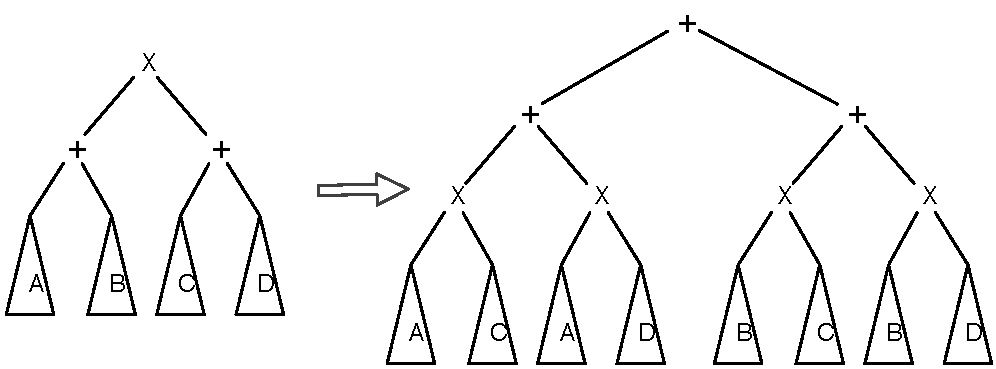
\includegraphics[width=.9\textwidth]{Fig/expression.pdf}
\caption{Distributing $\times$-node \label{fig:expr}}
\end{figure}
\end{solution}

%----------------------------------------------------------------------
\hdr{CS 573 HW0}{Zigang Xiao (zxiao2) HW0 \#5}
\item
\begin{enumerate}
\item
What is the \emph{exact} expected number of cards that Professor Jay hurls into the watermelon?

\item
For each of the statements below, give the \emph{exact} probability that the statement is true of the \EMPH{first} pair of cards Professor Jay turns over.
\begin{enumerate}
\item
Both cards are threes.
\item
One card is a three, and the other card is a club.
\item
If (at least) one card is a heart, then (at least) one card is a diamond.
\item
The card from the red deck has higher rank than the card from the blue deck.
\end{enumerate}

\item
For each of the statements below, give the \emph{exact} probability that the statement is true of the \EMPH{last} pair of cards Professor Jay turns over.
\begin{enumerate}
\item
Both cards are threes.
\item
One card is a three, and the other card is a club.
\item
If (at least) one card is a heart, then (at least) one card is a diamond.
\item
The card from the red deck has higher rank than the card from the blue deck.
\end{enumerate}
\end{enumerate}

\begin{solution}
\begin{enumerate}
\item 1751/52

\item
\begin{enumerate}
\item 1/169
\item 1/26
\item 11/16
\item 6/13
\end{enumerate}

\item
\begin{enumerate}
\item 7/103
\item 31/103
\item 77/103
\item 48/103
\end{enumerate}
\end{enumerate}
\end{solution}


%----------------------------------------------------------------------
\end{enumerate}

\textbf{Credit:} I had discussion with Leslie Hwang, Yuelin Du and Pei-Ci Wu
when working on this homework. Thanks to Mr. Qiang Ma for providing insightful
suggestion to the proof of problem 3.  
\end{document}

%----------------------------------------------------------------------

\begin{comment}
  For the \textsc{HighestToRight$(\ell)$} query, we first sort the the points
  according to their $x$-coordinates. Then, we build a binary tree from bottom
  up.  For each two nodes, we create a parent node for them. The coordinate of
  the child node that has greater $y$-coordinate will be stored in this parent
  node. The algorithm is described as follows: 

\begin{center}\small
\begin{algorithm}
\textul{$\mathsc{HighestToRight}(l)$:}\+
\\	$p \gets $ binary search for the point $(x,y)$ closest to $l$ in $x+$ direction,\+
\\      return \textsc{None} if every point in $S$ has $x$-coordinate less than $l$. \-
\\	if $p$ is \textsc{None}\+
\\		return \textsc{None}\-
\\	while $p$ is not root\+
\\		$q \gets parent(p)$
\\		if $q.x < p.x$\+
\\			break\-
\\		$p \gets q$\-
\\	return $p$
\end{algorithm}
\end{center}

\textbf{Analysis:} In the worst case the tree will be a complete binary tree. 
So the tree will have at most $2n-1$ node and use $O(n)$ space. 
The query uses a $O(lg(n))$ binary search and will trace from a bottom node to the root, 
which takes another $O(lg(n))$ time.
Hence the total time complexity of query will be in $O(lg(n))$.
  %When performing a query with parameter $l$, we first use a binary
  %search to locate the point $(x,y)$ such that $x>=l$ and closer to $l$ than
  %any other points in $x$-coordinate. Then we continue to 

Similarly, for \textsc{RIghtMostAbove$(\ell)$}, we can build another tree by
sorting in $y$-coordinates first and build a binary tree from bottom up.
\end{comment}
